\documentclass{article}
\usepackage{tikz}
\usepackage{pgfplots}
\pgfplotsset{compat=1.18}
\usetikzlibrary{patterns}

\begin{document}

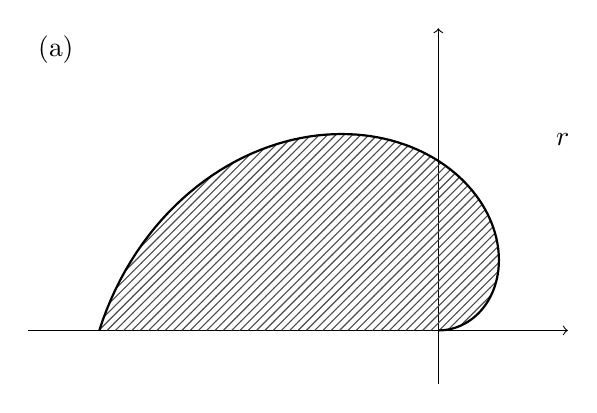
\begin{tikzpicture}
    \begin{axis}[
            axis lines=middle,
            axis line style={->},
            xmin=-3.8, xmax=1.2,
            ymin=-0.5, ymax=2.8,
            ticks=none,
            xlabel style={anchor=west},
            ylabel style={anchor=south},
            axis equal image
        ]

        % 1. Filled/Hatched region under the spiral curve
        \addplot[
            domain=0:pi,
            samples=100,
            pattern=north east lines,  % Hatching pattern
            pattern color=black!70,
            draw=none
        ]
        (
        {x*cos(deg(x))}, % Parametric x = r * cos(theta) = theta * cos(theta)
        {x*sin(deg(x))}  % Parametric y = r * sin(theta) = theta * sin(theta)
        )
        \closedcycle; % Closes path back along the x-axis to origin

        % 2. Outer spiral boundary curve
        \addplot[
            domain=0:pi,
            samples=100,
            thick,
            black
        ]
        (
        {x*cos(deg(x))},
        {x*sin(deg(x))}
        );

        % 3. Text Labels
        \node at (axis cs: -3.8, 2.6) [anchor=west] {(a)};
        \node at (axis cs: 1.0, 1.8) [anchor=west] {$r = \theta$};

    \end{axis}
\end{tikzpicture}

\end{document}